
        \documentclass[tikz]{standalone}
        \begin{document}
        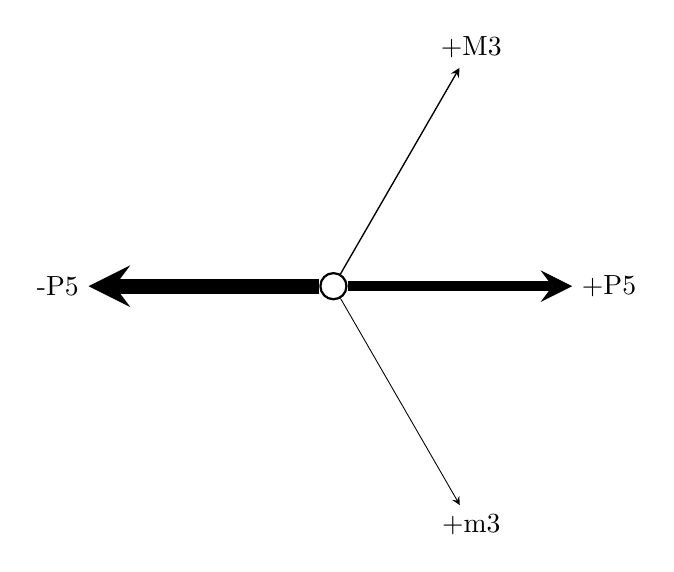
\begin{tikzpicture}[scale=3.5, ->, >=stealth]

        % the circle
        \node (origin) at (0,0) [draw,circle,black,fill=white,thick]{};
        % constant scaling for widths
        \def\cons{10}
        
                \node (0) at +(0*360/6:1) {+P5};
                \path (origin) edge [line width=\cons*0.3825754874465767] node {} (0);
                
                \node (1) at +(-1*360/6:1) {+m3};
                \path (origin) edge [line width=\cons*0.031649049986075976] node {} (1);
                
                \node (3) at +(-3*360/6:1) {-P5};
                \path (origin) edge [line width=\cons*0.5366596489839788] node {} (3);
                
                \node (5) at +(-5*360/6:1) {+M3};
                \path (origin) edge [line width=\cons*0.0491158135833684] node {} (5);
                
        \end{tikzpicture}
        \end{document}
        